% %\RequirePackage{lineno}
% 
% %\documentclass[aps,prb,superscriptaddress,showpacs,amsmath,amssymb,letterpaper,preprint]{revtex4}
% %\documentclass[aps,prb,superscriptaddress,showpacs,amsmath,amssymb,letterpaper]{revtex4}
% %\documentclass[aps,prb,superscriptaddress,showpacs,amsmath,amssymb,letterpaper,twocolumn]{revtex4}%floatfix
% 
% % https://authors.aps.org/revtex4/revtex4_faq.html#u1
% % use the following for a one-column, double-spaced, 12 pt document
% %\documentclass[preprint,prb,         showpacs,amsmath,amssymb]{revtex4-1}
% 
% % use the following for the published layout
% \documentclass[reprint,pra,         showpacs,amsmath,amssymb]{revtex4-1}
% 
% %For APS journals, only the prb option gives superscript-style citations.
% 
% \usepackage{mciteplus} % for bibliography style ``apsrevM''
% %\usepackage{dcolumn}
% \usepackage{graphicx}
% \usepackage{epsfig,color,verbatim} % multi-line comments
% \usepackage{subfigure}             % allows for use of "sub figure" 1a, 1b, etc
% \usepackage{hyperref}
% 
% %\linenumbers
% 
% \usepackage{amsmath} % advanced math
% \usepackage{appendix}
% %\usepackage[backref, colorlinks=false, pdftitle={Correction to the single scatterer quasi-1D models}, pdfauthor={Tom Mahler, Ben Payne, Alexey Yamilov}, pdfsubject={for publication}, pdfkeywords={localization, transmission, random, media}]{hyperref}
% \begin{document}
% 
\chapter{Near-field effects in wave transport through in disordered waveguides}
\label{chap:closed_channels}
\label{paper:3_start}

\begin{center}
Ben Payne$^1$, Tom Mahler$^1$, and Alexey Yamilov$^1$
\end{center}

\ \\
\begin{center}
\textit{$^1$Department of Physics, Missouri University of Science \& Technology,\\ Rolla, MO 65409}
%$^2$Department of Applied Physics, Yale University, New Haven, CT 06520}
\end{center}

\ \\
% \author{Ben~Payne, %\footnote{Electronic~address:~benjamin.payne@mst.edu},
% Tom~Mahler, %\footnote{Electronic~address:~tom.mahler@mst.edu},
% Alexey~G.~Yamilov\footnote{Electronic~address:~yamilov@mst.edu}}
% \affiliation{Department of Physics, Missouri University of 
% Science \& Technology, Rolla, MO 65409}
% \date{\today}
% 
% \begin{abstract}
\addcontentsline{toc}{section}{ABSTRACT}
\begin{center}\textbf{ABSTRACT\footnote{In preparation for Physical Review B (2012).}}        \end{center}

Evanescent coupling between scatterers in the course of wave propagation through random media is a notoriously difficult problem. Commonly these near-field effects are not considered explicitly. Instead, a phenomenological parameter, transport mean free path, is introduced. This treatment is sufficient to describe the macroscopic wave transport as exemplified by the success of Dorokhov and Mello, Pereyra, and Kumar (DMPK) theory. 
% 
% % OLD:
% %In models of transport in quasi-1D waveguides with random media such as that of Dorokhov and Mello, Pereyra, and Kumar, evanescent channels have been not included. Work by Bagwell and others has demonstrated that for a single scatterer inclusion of evanescent channels can be reduced to equivalent systems with only propagating channels, renormalizing scattering length. Here we show that evanescent channels can be analytically accounted for by renormalization of transfer matrices for multiple scatterers, thus including interaction and density. The role of evanescent channels is equivalent to renormalization of transport mean free path for systems with only propagating channels. Equivalence is determined by agreement with single parameter scaling; further, the entire distribution of conductance is correspondingly renormalized.
% 
% \pacs{42.25.Dd}
% % 42.25.Dd = Wave propagation in random media
% 
% \end{abstract}
% 
% \maketitle % declares end of title page
% 
% To cite:\cite{1999_van_Rossum,1995_Nieuwenhuizen,2007_Heinrichs,2004_Heinrichs,2003_Heinrichs,2002_Heinrichs}

%%%%%%%%%%%%%%%%%%%%%%%%%%%%%%%%%%%%%%%%%%%%%%%%%%%%%%%%%%%%%%%%%%%%%%%%%%%%%%
\section{INTRODUCTION}
%%%%%%%%%%%%%%%%%%%%%%%%%%%%%%%%%%%%%%%%%%%%%%%%%%%%%%%%%%%%%%%%%%%%%%%%%%%%%%
One approach to describing transport in waveguides is to define a set of discrete channels. This basis is useful since the transport properties can then be calculated in terms of channels and converted to spatially-resolved values.

Evanescent channels are usually neglected in calculations of conductivity with passive media since the wave propagation decays exponentially~\cite{1982_Dorokhov_DMPK,1988_Mello_Kumar_DMPK}. Another justification is that if the field detector is far from the media then the evanescent channels will not be measured and cannot contribute significantly to propagation properties. These two arguments are distinct as the first applies to interscatterer transport, whereas the second applies to measurements outside the sample. Inside the medium it has been shown for single scatterers~\cite{1990_Bagwell,1991_Kumar_Bagwell} that not including evanescent channels is equivalent to renormalizing scattering length. Additionally, if the density of scatterers is low enough, then there is sufficient separation between scatterers that evanescent channels do not contribute to interaction. 

Our motivation in revisiting the issue of evanescent channels is two-fold. First, when studying the regime of Anderson localization~\cite{1958_Anderson,2009_Lagendijk_PT,2010_Abrahams} scatterers are densely packed~\cite{1960_Ioffe_criterion}. Second, we have developed a numerical model to investigate propagation of light waves which can include gain and absorption; evanescent waves may be expected to play an important role in media with gain.
%light rather than electron propagation. Our model does not include electron-electron interference.
Optical gain enhances interaction between scatterers~\cite{2006_Heinrichs,1997_Heinrichs}, so the importance of evanescent channels will increase in multiply-scattering media. In this letter, only passive media are considered; the role of gain (and absorption) will be presented separately. 


This letter covers passive random disorder and multiple scatterers, which is treated theoretically by Dorokhov~\cite{1982_Dorokhov_DMPK} and Mello, Pereyra, and Kumar~\cite{1988_Mello_Kumar_DMPK} (DMPK). For waveguides DMPK theory assumes (1) all propagating channels are the same, % page 297, after eq 2.36 of \cite{1988_Mello_Kumar_DMPK}
 and (2) evanescent channels are not included. % page 292
We have previously found that propagating channels are not equivalent~\cite{2008_Yamilov_PRB}, and here show that evanescent channels do have a role in conductance. Compared to a system with only propagating channels, including evanescent channels is equivalent to renormalizing transport mean free path $\ell_{\rm tmfp}$. The renormalization does not effect the validity single parameter scaling~\cite{1979_Anderson}.

The transfer matrix method~\cite{1981_MacKinnon_scaling,1992_Pendry,2003_Kettemann} used in our numerical model requires the presence of evanescent channels to be explicitly included, whereas DMPK specifically excludes them. A third class of models implicitly include evanescent channels; for example the position-dependent diffusion coefficient~\cite{2000_van_Tiggelen,2007_Skipetrov}, finite-difference time-domain simulations, and descriptions using the local density of states~\cite{2006_vanTiggelen,2010_Mosk_Skipetrov_PRL,2002_Chicanne}. These include evanescent channels because the channels carry energy.

The quasi-one dimensional (quasi-1D) geometry of a waveguide is useful for studying wave transport because transverse channels are quantized. The component of wave number $k = \omega/c$ perpendicular to the direction of propagation is $k_{\perp n}=(n \pi)/W$, where $W$ is the width of the waveguide, $n$ is the channel index, $\omega$ is frequency, and $c$ is the speed of the wave. The component of $k$ parallel to the direction of propagation, $k_{\parallel n}=\sqrt{(\omega/c)^2-\left(n \pi/W\right) ^2}$, can have imaginary values for sufficiently large channel index $n$ with fixed $W$. Here width $W$ is chosen such that the system is not close to the singularity $k_{\parallel}=0$~\cite{2008_Engheta_PRL}.
Channels with real-valued $k_{\parallel n}$  are ``open''  when the waveguide is empty, and channels for which $k_{\parallel}$ is imaginary are referred to as ``closed.'' For waveguides with scatterers, channels either propagating or evanescent, respectively.

Since work on including evanescent channels has been done previously for single scatterers~\cite{1990_Bagwell,2007_Froufe-Perez_PRE} and results of DMPK are well demonstrated~\cite{1997_Beenakker}, the purpose of this paper is to bridge the gap between renormalization of scattering length $\ell$ and $\ell_{\rm tmfp}$. Physically, $\ell$ characterizes the exponential decay length of ballistic attenuation whereas $\ell_{\rm tmfp}$ is the distance over which direction of propagation is randomized. For strongly scattering media, $\ell_{\rm tmfp} \approx \ell$; otherwise $\ell_{\rm tmfp} = \ell/(1-\langle \cos \theta \rangle)$ in bulk media. This reduces to $\ell_{\rm tmfp} = \ell/\left(1-\langle k_{\parallel n}/k\rangle \right)$ for quasi-1D systems since only discrete directions are available. Isotropic scattering in quasi-1D means $\ell_{\rm tmfp} = \ell$ when no closed channels are present. However renormalization of $\ell_{\rm tmfp}$ cannot be extrapolated from a single scatterer because $\ell$ does not account for interaction between scatterers. The $\ell_{\rm tmfp}$ is a function of scatterer density, scattering strength, waveguide width, and number of evanescent channels.


In this paper near-field analysis of single scatterers is quickly reviewed, then coupling of two scatterers by evanescent channels is studied analytically in Section~\ref{sec:renormalization}. In Section~\ref{sec:scatlength} the scattering length definition is modified by inclusion of evanescent channels. A robust numerical model is described in Section~\ref{sec:numericalSim}, then simulation results are presented in Section~\ref{sec:numericalResults}. Numeric modeling of multiple scatterers demonstrates the effect of including evanescent channels while maintaining single parameter scaling by renormalization of $\ell_{\rm tmfp}$. 

%The numerical model is developed in section III, which uses randomly placed scattering potentials in a planar quasi-1D metallic waveguide. The transfer matrix method is used~\cite{1981_MacKinnon_scaling,1992_Pendry,2003_Kettemann}, and self-embedding technique \cite{1999_yamilov_selfembed,1976_Bellman_Wing_embedding} extends the limits of numerically accurate simulation by renormalization of eigenvalues. The number of propagating and evanescent channels, scattering strength, system dimensions, and scatterer density are adjustable parameters. The results are transmission and reflection matrices, and many realizations are ensemble averaged to yield statistical behavior. 

%%%%%%%%%%%%%%%%%%%%%%%%%%%%%%%%%%%%%%%%%%%%%%%%%%%%%%%%%%%%%%%%%%%%%%%%%%%%%%
\section{ANALYTICAL RENORMALIZATION OF SCATTERERS WITH EVANESCENT CHANNELS}
\label{sec:renormalization}
%%%%%%%%%%%%%%%%%%%%%%%%%%%%%%%%%%%%%%%%%%%%%%%%%%%%%%%%%%%%%%%%%%%%%%%%%%%%%%

% folding technique puts the evanescent channel information in the propagating channels. 
% ``Folding'' is actually just partially solving homogeneous linear equations.

When modeling waveguides with disorder, a single scatterer is described by transfer matrices~\cite{1981_MacKinnon_scaling,1992_Pendry,2003_Kettemann}
% note: when MacKinnon cites tmm, he uses 1981_MacKinnon_scaling and 
% MacKinnon A 1994 J. Phys. Condensed Matter 6, 2511
with the strength of the scatterer and position as parameters. The effect of additional scatterers on transport properties cannot be extrapolated from this information since there are no parameters for interaction between scatterers. A minimum of two scatterers are needed to correctly account for interaction and scatterer density. 

For system with multiple scatterers, each single scattering matrix can be analytically reduced from rank $2(N_p+N_e)$ to $2 N_p$, where $N_p$ and $N_e$ are the number of propagating and evanescent channels respectively, by applying the boundary condition of no transmission from evanescent channels~\cite{1990_Bagwell}. This partial solving of the linear set of equations is referred to as ``folding,'' as the algorithm recursively folds information into other matrix elements resulting in reduced rank.  There is conservation of information in that the information stored in the original rank $2(N_p+N_e)$ matrix is still contained within the new ``folded'' rank $2N_p$ matrix, albeit with increasingly complicated elements.  By induction (using the developed recursion relation) a matrix of rank $2N_p$ can account for $N_p$ propagating channels and an infinite number of evanescent channels. % The result differs from Ref.~\citenum{1990_Bagwell} and is a more explicit reworking of Ref.~\citenum{1991_Kumar_Bagwell}. The derivation explains the renormalization of conductance for multiple scatterers shown by the numerical model.


In the transfer matrix approach, Bagwell and coworkers~\cite{1990_Bagwell,1991_Kumar_Bagwell} have shown the scattering matrix can be ``folded,'' reducing the rank from $2(N_p+N_e)$ to $2N_p$. The scattering matrix $\Gamma$ is related to the scattering length by 
%\begin{equation}
$\ell^{(M)} = 1/\left(\sum_{a,b} \frac{1}{4} \frac{1}{d} \frac{1}{k_{\parallel a} k_{\parallel b}} \langle \Gamma_{a,b}^2 \rangle\right)$ where $a$, $b$ are input, output channels and $d$ is average separation between scatterers along the direction of propagation~\cite{2007_Froufe-Perez_PRE}. The $\langle \cdots \rangle$ denotes an average over a disordered ensemble,
%\label{eq:l_scat_mello_analytical}
% Eq. 3.36 of PRE 75 031113 2007
% Eq 13 of Physica A v386, 2007
%\end{equation}
%where $\hat{\Gamma}$ is the scattering matrix. 
Similar analytic ``folding'' of scattering matrices applies to multiple scatterers. Folding the matrix for a single scatterer has scatterer strength as a parameter, and for multiple scatterers an additional parameter is introduced: interaction between adjacent scatterers. The interaction between scatterers is where the effect of evanescent channels becomes relevant to transport. In order to model interaction of scatterers by both the propagating and evanescent channels, the reduced transfer matrices for at minimum two scatterers needs to be derived, as is done in Ref.~\citenum{2007_Froufe-Perez_PhysA}.



Here we assume transmission information will be a far-field measurement (no transmission measured in evanescent channels). Then there are two distinct methods of applying the folding algorithm. In the first method, the rank of each scatterer matrix is reduced analytically to propagating channels only, then standard matrix multiplication of the scatterer and free space matrices (which are also rank $2N_p$ and do not need to be folded) is performed~\cite{2004_Mello_Kumar_book}. The second method is to perform the multiplications of scatterer and free space matrices with evanescent channels, then fold (analytically reduce) the product. Between these two extrema are compromises of varying order; for instance folding pairs of scatterers, or three scatterers. The question arises  as to whether folding the product is equivalent to folding each matrix, or some subset of matrices. Mathematically, the two are not equal, since the operation of ``fold then multiply'' loses information about transport by evanescent channels. %However, folding then multiplying is faster since the matrices are of lower rank, and also remain numerically stable for more multiplications.

The first method, ``fold-combine,'' is computationally desirable since the transfer matrices being multiplied are of lower rank, translating to slower growth in numerical error and faster computation. Although the folding procedure conserves information for each scattering matrix, information about density (interaction between scatterers) is lost in propagation. The second approach, ``combine-fold,'' loses no information. The propagation includes all channel information, and folding occurs after the total propagation matrix is known.

%in pseudo-math, let $F$ be the free space matrix and let $T$ be the scattering matrix. Compare\\ $F*fold(T)*F*fold(T)*F*fold(T)*F*fold(T)*F*fold(T)*F$ versus\\ $F*fold(T*F*T)*F*fold(T*F*T)*F$ versus\\ $fold(F*T*F*T*F*T*F*T*F)$

This question of equivalence of folding and multiplying order is addressed using an analytical model comparing two scatterers. A finite number of propagating and evanescent channels is modeled. The separation between the two scatterers is fixed and interaction strength is varied.
%Here there should be results from the Mathematica code, showing when combine-fold versus fold-combine breaks down for varying separation. 

The result from this analytical two-scatterer model is that interaction between scatterers in evanescent channels does play a role in transport for sufficient interaction strength. However, transport models with no evanescent channels such as DMPK have successfully matched experiments by using~$\ell_{\rm tmfp}$ as a fitting parameter. This is probably due to systems being in the density regime where the single scatterer approximation is valid. Then the density~$d$ and scattering cross-section~$\sigma$ yield~$\ell_{\rm tmfp}=1/(d\ \sigma)$, where scattering cross-section is proportional to the square of scatterer strength. However, for sufficiently dense or strong scattering, $\ell_{\rm tmfp}$ is not characterized by that relation since the single scattering approximation is invalid. In this new regime adjacent scatterers are coupled by evanescent channels.

\section{RENORMALIZATION OF SCATTERING LENGTH DUE TO \\EVANESCENT CHANNELS}
\label{sec:scatlength}

In this section we show, using an analytical model of two scatterers in a quasi-1D waveguide, that scattering length is renormalized by inclusion of evanescent channels. This system is in the ballistic regime since there is very little scattering between channels; transmission matrices with diagonal elements of roughly unity are found. This is an independent numerical validation of the folding procedure of the previous section.


The scattering length characterizes exponential attenuation of intensity for a ballistic source. In a quasi-1D waveguide, this decay length is distinct for each channel. Thus although the ballistic component is similar to a single exponential decay, it is actually an accumulation of the contributions of each channel. This can be observed by fitting the ballistic component of the conductance $g_b$ with 
\begin{equation}
g_{\rm b}= \sum_{a=}^{N_p}\sum_{b=1}^{N_p} \left| \langle t_{a,b} \rangle \right|^2 = \sum_{n=1}^{N_p} \exp\left(\frac{-L}{\ell \ k_{\parallel n}/k} \right)
\label{eq:gb_lscat}
\end{equation}
Here $\langle \cdots \rangle$ again refers to the average over a disordered ensemble, $t_{a,b}$ are elements of the complex-valued transmission matrix, and $L$ is the length of the waveguide.


An alternative (non-equivalent) definition of scattering length for any incident channel $a$ by measuring the reflection in channels~$b$ has been defined by Mello \textit{et al}~\cite{2007_Froufe-Perez_PhysA} to be
\begin{equation}
 \ell^{(M)} = \frac{N_p\ d}{\sum_{a,b} \left\langle R_{a,b} \right\rangle}
\label{eq:l_scat_mello_numerical}
% equation 3.36, page 8
% applied to Reflection matrix data from F90 quasi-1D code
% Eq 3.34 of PRE v75 031113, 2007
% Eq 13 of Physica A v386, 2007
%\begin{equation}
% $\ell=\sum_a \ell_{a}$.
% Eq 24 of Physica A v386, 2007
%\end{equation}
%The need to find scattering length for a given input channel means the ballistic transmission $T_a$ cannot be lumped together with the scattered transmission $T_{b\neq a}$. %This is the difference between $\ell_{a}^{(Y)}$ and $\ell_{a}^{(M)}$; the unjustifiable discard of $T_{b\neq a}$. \textbf{Needs to be verified analytically or numerically.}
\end{equation}
Here $\ell^{(M)}$ is the scattering length in terms of the reflection matrix elements $R_{a,b}$ summed over $N_p$ incident channels $a$ and $N_p$ output channels $b$, with the average distance $d$ between scatterers along the axis of propagation.
This definition can be used analytically, solving for $R$ with one or two scatterers and few channels, and used with a numerical model since the reflection matrix for and arbitrary number of scatterers and channels can be found for an ensemble of scatterer positions. 


% the discussion by mello of expansion terms is on page 8 of PRE v75 031113, 2007; specifically line 1 of column 1 on page 8; also Eq 3.29
% also Eq 14 of Physica A v386, 2007

The reflection matrix can be approximated as an expansion about $\varepsilon$; the second order correction includes propagating channels only. Here we find the third order corrections to $R_{a,b}$ and thus include evanescent channels. When scatterer strength averages to zero, then the third order correction of the expansion is zero. Thus, for electronic systems the renormalization of $\ell$ due to evanescent channels is smaller than photonic systems.

To find the expansion of $R$ we start with a single scattering matrix which includes evanescent channels. Each element in the matrix is of the form $\varepsilon \Gamma_{a,b}$ (input channel $a$, output channel $b$). This matrix is reduced in rank using the folding procedure leaving just propagating channels. Reflection matrix $R$ is calculated using the folded scattering matrix, then we let $\varepsilon \rightarrow 0$ and find the series expansion of $R$. The zero$^{th}$-order term of the expansion is 0 since as scattering strength goes to 0 then $R$ goes to 0. The first order term is also 0 when average scattering strength is 0, as for scattering in electronic systems. 

In photonic transport the first non-zero term of the expansion is of second order, which includes only propagating channel elements from the scattering matrix. The third-order term of expansion of $R$ contains the evanescent channel tunneling:
\begin{equation}
\frac{1}{4} \Gamma_{i_p,j_p}^2 \varepsilon ^2-\frac{1}{4} \left(\Gamma_{i_p,j_p} \Gamma_{i_p,j_e} \Gamma_{i_e,j_p}\right) \varepsilon ^3+O[\varepsilon^4 ].
\label{eq:expansion_of_R}
\end{equation}
% from /svn/research/quasi1d/quasi1d_two_scatterer/quasi1d_single_scatterer_folded.nb
In the second and third order terms (as denoted by $\varepsilon$), we have $\Gamma_{i_p,i_p'}$ for flux from propagating channel $i_p$ to propagating channel $i_p'$. The other two factors in the third order term represent ``propagating-to-evanescent'' and ``evanescent-to-propagating'' channel mixing. Higher order expansion terms have more complex tunneling sequences, all of which include evanescent channels. Our expansion can be used to predict the coupling sequences for any number of propagating and evanescent channels, and for any order of $\varepsilon$. 

In contrast to photonic transport, media scattering electrons have first and second-order terms which do not depend on evanescent channels. This demonstrates why systems describing electron transport may be less sensitive to evanescent channels. %In photonic transport, no attractive scatterers result in all odd powers of the expansion being zero (\textbf{Eq.~\ref{eq:expansion_of_R} contradicts this}), thus evanescent channels play a more important role in describing propagation.

There are four important assumptions in $\ell^{(M)}$: (1) the single scatter approximation, (2) the weak scattering approximation, (3) all reflected flux is ballistic, and (4) the inverse scattering length is average of the inverse scattering lengths per channel. The single scatterer approximation is based on the assumption that each scattering event can be treated individually. Scatterers are sufficiently far apart such that evanescent channel contributions are negligible. However, if scatterers in a finite waveguide have perfectly random positions, then there is a significant chance that there will be two adjacent  scatterers sufficiently close to void the single scatterer approximation.  

One can have random scatterer position while maintaining minimum  separation by ensuring that no two adjacent scatterers are closer than $\sqrt{W \ L/M}$, where $M$ is the number of scatterers. This requirement becomes exponentially harder as the number of scatterers is increased for a given area. %Computationally, more time is spent in medium creation due to the attempted placement of the last few scatterers.

Separation between scatterers deserves clarification on whether one means the separation along the propagation axis, as prescribed by Mello, or the actual separation distance between scatterers $D=\sqrt{z^2+y^2}$ which is to relevant to wave interaction. For quasi-1D systems, the separation along the z-axis $d$ is used in scattering length Eq.~\ref{eq:expansion_of_R}. In the analytic two-scatterer model, one can fix~$d$ or the absolute separation~$D$. When~$D$ is fixed, then $d=D \sin(\phi)$. To compare $d$ used in the analytical model to density of the numeric model, the average propagation distance $\langle d \rangle=L/M$ is used, with a minimum $D=\sqrt{W\ L/M}$.

The second assumption of $\ell^{(M)}$ is the weak scattering approximation ($|\Gamma_{a,b}|^2<<k_{\parallel a}k_{\parallel b}$ 
%eq 3.17 
in Ref.~\citenum{2007_Froufe-Perez_PRE}). This breaks down in the presence of evanescent channels since scattering light into a evanescent channel is equivalent to having a stronger scatterer. The purpose of assuming weak scatterers is to be able to neglect the contribution of non-incident transmission channels. 

The third assumption of Eq.~\ref{eq:l_scat_mello_numerical} is that all reflected flux is ballistic. This definition neglects flux transmitted in non-incident channels.
%\begin{equation}
%\frac{1}{\ell_{a}^{(Y)}} = \frac{1}{dz} \left\langle \sum_b R_{a,b} + \sum_{b \neq a} T_{a,b} \right\rangle  = \frac{1}{dz} \left\langle 2 \sum_b R_{a,b}  - T_{a,a} \right\rangle
%\end{equation}
Each scatterer distributes flux isotropically into channels, thus $R_{a,b}=T_{a,b}$ for $b \neq a$. %$\ell_{a,b}$ is the scattering length of channel~$b$ when light is incident in channel~$a$. There is a $\ell$ associated with each interior channel. When a single subscript is given, such as $\ell_{a}$, this denotes the scattering length of channel incident~$a$ summed over all interior channels. 
Further, the flux transmitted in the incident channel ($T_{a,a}$) is composed of ballistic and non-ballistic components (distinguishable by the consistency of the phase). Thus, to account for all the ballistic components of flux, the denominator of Eq.~\ref{eq:l_scat_mello_numerical} should be doubled.
%However, the non-incident transmission and reflection have equal probability. Thus $\ell_{a}^{Y)}$ is gives a better measure of the actual scattering length. 

Lastly (assumption four), by expanding the summation in Eq.~\ref{eq:gb_lscat} for channels $n$, it is apparent that $1/\ell\neq\sum_n (1/\ell_n)$, where $\ell_n = \ell\ k_{\parallel n}/k$. There is an exponential decay associated with each channel, characterized by $\ell_n$. The complete ballistic component is then a sum of the attenuating flux.

% larger channels have slower wave propagation, leading to longer interaction time. Longer interaction time is equivalent to stronger scattering, making the weak scattering approximation less valid. Lowering the scattering strength while maintaining $\langle \alpha \rangle =0$ decreases the difference between the two lengths.

Now that the scattering length has been discussed for few scatterers, the next progression is to a many scatterer system, where transport mean free path is relevant. To better understand the role of evanescent channels in real systems, a numerical model described below is used in order to simulate thousands of scatters (instead of a few). The analytical folding technique described above is not used in the numerical simulation of  evanescent channels. The purpose of investigating the folding algorithm was to measure interaction between scatterers and renormalization of multiple-scatterer lengths. 



%%%%%%%%%%%%%%%%%%%%%%%%%%%%%%%%%%%%%%%%%%%%%%%%%%%%%%%%%%%%%%%%%%%%%%%%%%%%%%
\section{NUMERICAL SIMULATION MODEL DESCRIPTION}
\label{sec:numericalSim}
%%%%%%%%%%%%%%%%%%%%%%%%%%%%%%%%%%%%%%%%%%%%%%%%%%%%%%%%%%%%%%%%%%%%%%%%%%%%%%

An \textit{ab initio} numerical model based on the Helmholtz equation is used to investigate wave transport in a waveguide with many scatterers. The second-order differential wave equation for the $s$-polarized electric field is solved using the transfer matrix method~\cite{1981_MacKinnon_scaling,1992_Pendry,2003_Kettemann}. Initially a point scatterer of strength $\alpha$ is introduced at position $y_0$, $z_0$ in the waveguide by replacing the dielectric $\epsilon=1$ with $\epsilon = 1+ \alpha\ \delta(y-y_0,z-z_0)$. When strength parameter $\alpha$ is real then the medium is passive (no energy lost or gained). Two types of transfer matrices are developed in this section: one which matches the electric field and derivative of field before and after the scatterer, and one which propagates the field through an empty waveguide over the distance between scatterers. To fully resolve the $\delta$ function using discrete channels transfer matrices would need to have infinite rank ($N_p$ propagation channels plus an infinite number of evanescent channels $N_e$). By including only a finite number of evanescent channels the effective dielectric for each scatterer is a finite sum of Fourier components $1+ \alpha \sum f_n(y_0)$ for $N_p+N_e$ channels. Thus the numeric model has scattering potentials rather than point scatterers. The number of propagating channels $N_p$ depends on the width of the waveguide, and the number of evanescent channels $N_e$ is a freely adjustable parameter.

\subsection{Effective Refractive Index}
Models of electronic systems have scatterers whose average strength is zero (attractive and repulsive scatterers)~\cite{2007_Froufe-Perez_PRE}. In contrast, photonic systems have scatterers which are only repulsive. The numerical model presented here can have any distribution of scatterer strength by setting $\alpha$ to be a positive or negative fixed value with equal probability (binary distribution for electronic), or the scatterers can be of fixed strength (photonic) with constant $\alpha$. When average scattering strength is zero the effective refractive index of the medium is $n=1$ since we assume empty space between scattering potentials. (The motivation for this choice is that when gain is later added, we want to avoid lasing in a media without scatterers.) 

When average scattering strength $\langle \alpha \rangle$ is not zero, then the refractive index is changed by the following amount. Assuming there are $M$ $\delta$-function scatterers each with strength $\alpha$, the Sellmeier equation for average dielectric is
%\begin{equation}
$\overline{\epsilon} = 1+\alpha \sum_{i=1}^M \delta(z-z_i,y-y_i)$.
%\end{equation}
To eliminate the $\delta$ function in the limit of a large waveguide, integrate over the area of the waveguide and 
%\begin{equation}
%\int_0^L \int_0^W \overline{\epsilon}\ dz\ dy = \int_0^L \int_0^W \left(1+\alpha \sum_{i=1}^M \delta(z-z_i,y-y_i)\right)dz\ dy.
%\end{equation}
normalize both sides by waveguide area $LW$; then the effective dielectric constant is 
%\begin{equation}
$\overline{\epsilon} = 1 + \alpha \frac{M}{LW}$
%\end{equation}
Since a finite number of evanescent channels are included, the actual value is closer to unity. For a specific waveguide configuration the refractive index can be found by summing the aforementioned Fourier components and averaging over all scatterer positions. This effective refractive index $\eta=\sqrt{\epsilon}$ has the effect of making the wavelength smaller by $\lambda = \lambda_0/\eta$. 

%Vellekoop~\cite{2008_Vellekoop} writes that the effective number of propagating channels scales as the dielectric constant. % see page 107
% this does not match style of referencing other papers
%Thus the number of effective propagating channels in a waveguide depends on width $W$ and the (non-zero average) strength of the scatterers. Arguments are also given as to why the change in effective number of channels do not change the transport properties. Our numerical results bear these assumptions out; it appears only effective density of scatterers $\alpha \frac{M}{LW}$ matters, not the average scatterer strength $\langle \alpha \rangle$. The numerical results in section V have fixed scatterer strength $\alpha=1$; not shown are the similar results for $\langle \alpha \rangle=0$.
%\textbf{[This does not specify that the values are slightly off-set, indicating an effective number of channels?]}

\subsection{Transfer Matrices}
Scatterering in the waveguide is determined by a scattering potential; then propagation of electric field through the quasi-1D waveguide is described using transfer matrices~\cite{2004_Mello_Kumar_book}.
%Start with the vector $\vec{v}(0)$, which describes $N_p$ and $N_e$ channels for both the electric field and the field derivative, total length $2(N_p+N_e)$, on the incident side of the medium.  There is a similar vector on the other side of the quasi-1D waveguide, $\vec{v}(L)$, of the same size. For $\vec{v}(0)$, assume an input beam in the $N_p^{th}$ channel. (Later on the input channel will be iterated over all propagating channels. The input could be to evanescent channels, but that is not investigated in this letter.)
The rank of the matrices is dependent on the number of propagating and evanescent channels of the waveguide.  Electric field $E$ and its derivative $dE/dz=E'$ in propagating channels moving through distance $\Delta z$ in free space are found from the solution to the wave equation for the $n^{th}$ channel:
%\begin{widetext}
\begin{equation}
\begin{gathered}
E_n(z+q)=E_n(z)\cos(k_{\parallel n}q)+k_{\parallel n}^{-1}
E_n^{'}(z)\sin(k_{\parallel n}q) \\
k_{\parallel n}^{-1}E_n^{'}(z+q)=-E_n(z)\sin(k_{\parallel n} q)
+k_{\parallel n}^{-1}E_n^{'}(z)\cos(k_{\parallel n}q)
\end{gathered}
\label{eq:electricfield}
\end{equation}
%\end{widetext}
For evanescent channels in free space the equations are similar to Eq.~\ref{eq:electricfield} except $k$ is replaced by the imaginary $i \kappa$ and hyperbolic functions are used. 
\begin{comment}
% REDUNDANT
\begin{equation}
\begin{gathered}
E_n(z+q)=E_n(z)\cosh(\kappa_{\parallel n}q)+
\kappa_{\parallel n}^{-1}E_n^{'}(z)\sinh(\kappa_{\parallel n}q)\\
\kappa_{\parallel n}^{-1}E_n^{'}(z+q)=E_n(z)\sinh(\kappa_{\parallel n}
q)+\kappa_{\parallel n}^{-1}E_n^{'}(z)\cos(\kappa_{\parallel n}q)
\end{gathered}
\end{equation}
\end{comment}
These sets of equations form a free space matrix of $2\ (N_p+N_c)$ by $2\ (N_p+N_c)$ which depends on distance $p$ (between scatterers). 

A second matrix is needed for translation of $E$ and $E'$ across the scattering potential. The electric field before and after each scattering potential must be equal, $E_n(z+\Delta)=E_n(z)$, in the limit that $\Delta \rightarrow 0$. The first derivative is 
%\begin{widetext}
\begin{equation}
E_n^{'}(z+\Delta)=E_n^{'}(z)-\alpha\left(\frac{\omega^2}{c^2}\right)\sum_{m=1}^{N_p+N_e}
\frac{2}{W}\sin(k_{\perp n}y)\sin(k_{\perp m}y) E_m(z)
\label{eq:scattering_lines} 
\end{equation}
%\end{widetext}
%where
%\begin{equation}
%A_{nm}=\frac{2}{W}sin(k_{\perp n}y)sin(k_{\perp m}y)
%\end{equation}
%The coefficient $\alpha$ describes the scattering strength of the scatterers. 
The channel-indexed equations can be written as a set of linear equations; thus wave propagation can be described by matrices of rank $2 (N_p+N_e)$ of two types: free space matrices (Eq.~\ref{eq:electricfield}) and scattering matrices (Eq.~\ref{eq:scattering_lines}; second term defines $\Gamma_{m,n}$).  These matrices (c.f.~Fig.~\ref{fig:tomsmatrices}) are multiplied to form a total matrix which describes propagation of the continuous wave (CW) electric field through the waveguide. This transfer matrix method can be used to calculate the reflection and transmission coefficients for each channel. 

When choosing the width of the waveguide, a singularity of wave speed occurs for certain $W$ since the speed of transmission is zero for the largest channel ($k_{\parallel,n=N_p}=0$). %[Strange things happen, since the interaction time with the scatterer is infinite.}~\cite{1990_Bagwell}] 
To avoid this phenomenon we set $W = (N_p+1/2)\lambda/2$. The offset of $N_p$ by half puts the width between singularities~\cite{2008_Engheta_PRL}. % valid only for <\alpha>\neq0?
% same as Eq 3.64 of PRE 75 031113 2007

\begin{figure}
(a)
\hskip -.3in
%\begin{flushleft}(a)\end{flushleft}
%\vskip -0.5cm
\centerline{
\scalebox{.4}{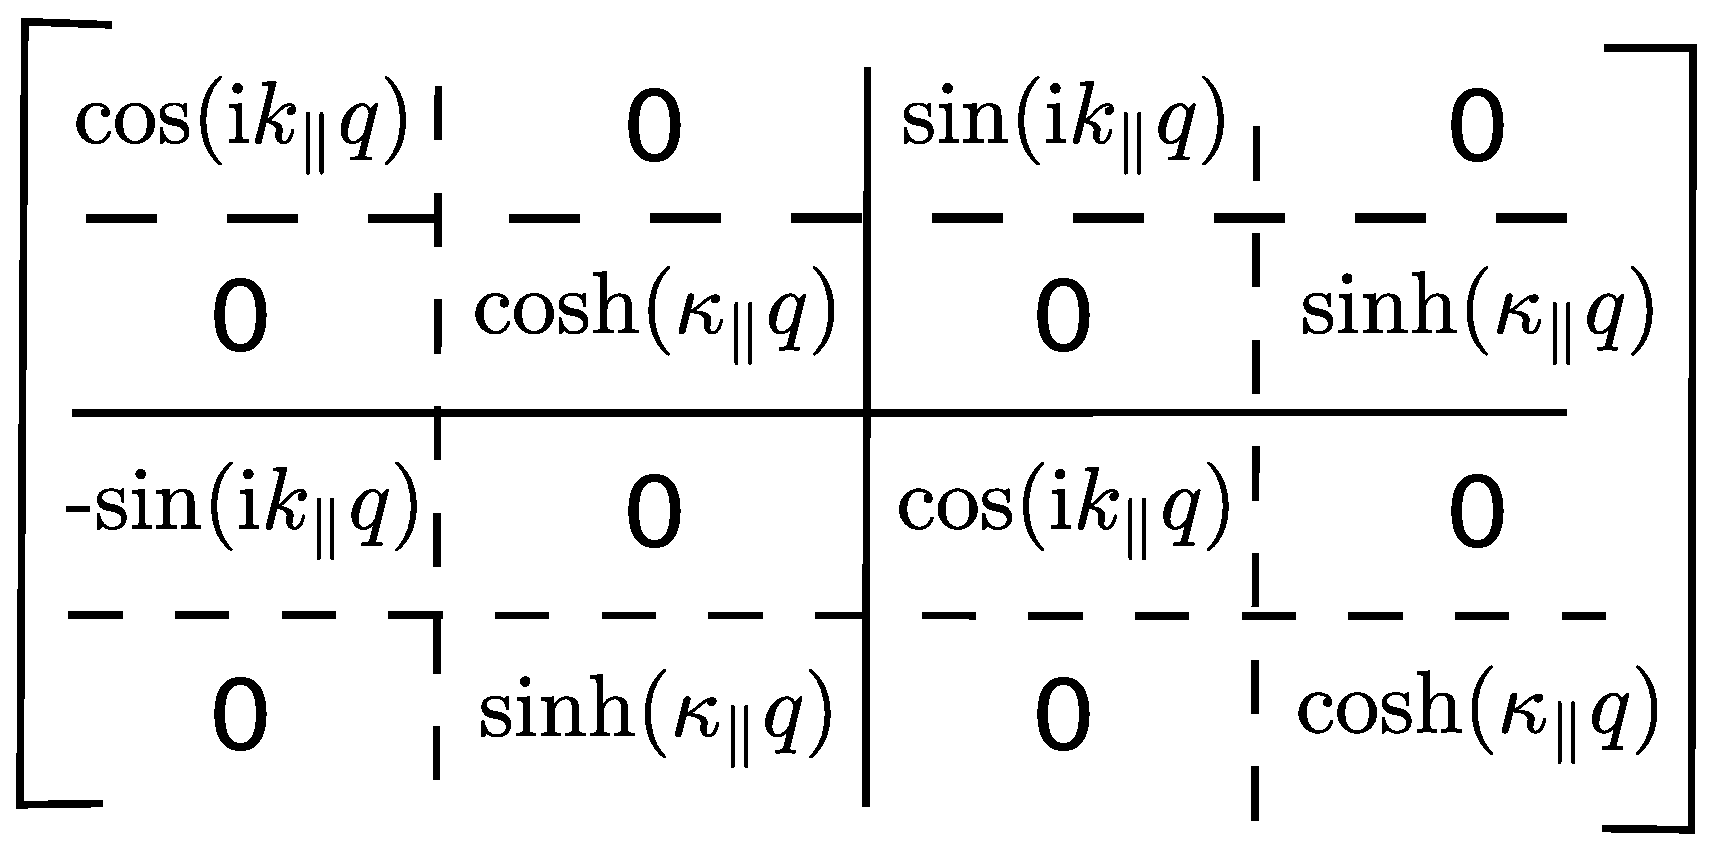
\includegraphics[height=3.9in]{chapters/Near-field_effects_in_wave_transport_through_in_disordered_waveguides/pictures/propagation_matrix_vector}}
%\begin{flushleft}(b)\end{flushleft}
\ (b)\ 
%\vskip -0.5cm
\scalebox{.5}{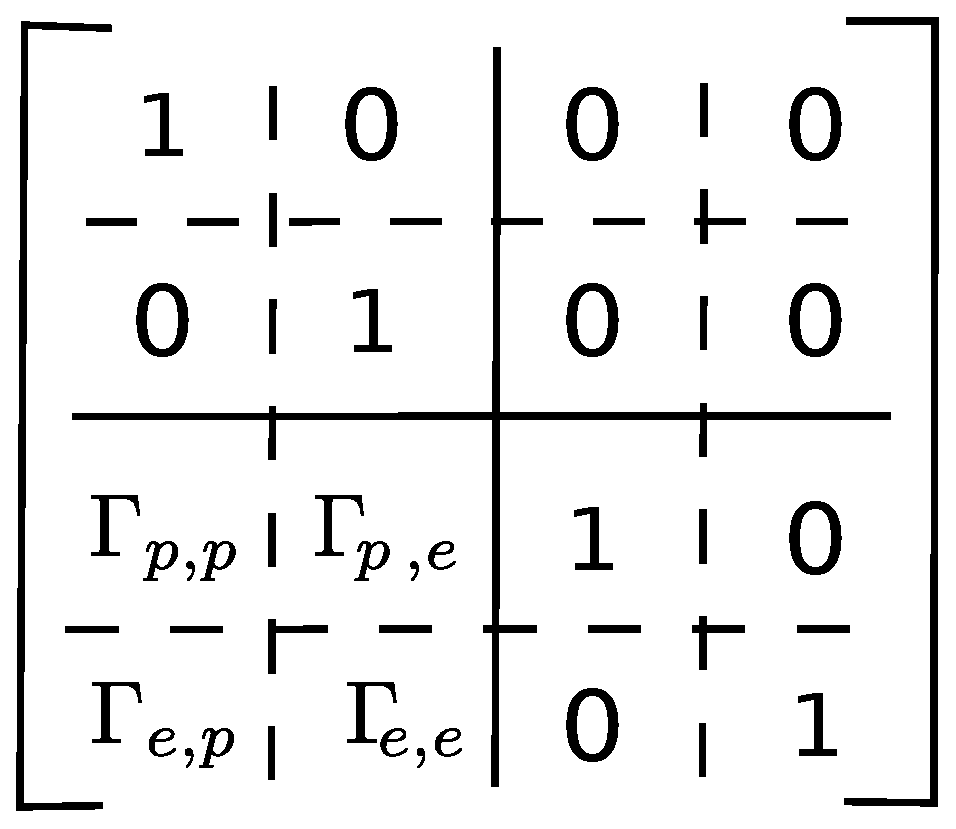
\includegraphics[height=3in]{chapters/Near-field_effects_in_wave_transport_through_in_disordered_waveguides/pictures/scattering_matrix_vector}}
}
\caption[(a) General form of empty waveguide transfer matrices for propagation of electric field $E$ and $E'$ over distance $\Delta z$ between scatterers.]{(a) General form of empty waveguide transfer matrices for propagation of electric field $E$ and $E'$ over distance $\Delta z$ between scatterers. (b) Scattering matrices, based on Eq.~\ref{eq:scattering_lines}, where $\Gamma_{nm}$ denotes non-zero terms which can be complex valued. Each matrix is separated into four $N_p+N_e $x$ N_p+N_e$ quadrants (long dashed lines), each containing information from propagating-to-propagating channels (upper left short-dashed subquadrants) as well as evanescent-to-evanescent (lower right short dashed subquadrants). }
\label{fig:tomsmatrices}
\end{figure}

%%%%%%%%%%%%%%%%%%%%%%%%%%%%%%%%%%%%%%%%%%%%%%%%%%%%%%%%%%%%%%%%%%%%%%%%%%%%%%
\subsection{Self-Embedding}
%%%%%%%%%%%%%%%%%%%%%%%%%%%%%%%%%%%%%%%%%%%%%%%%%%%%%%%%%%%%%%%%%%%%%%%%%%%%%%

%Due to the numerical instability which builds up in models of waveguides with many scatterers, 
The computation of the simple product of individual matrices is a straight-forward approach to field propagation but is not numerically stable over many multiplications, as the eigenvalues in the product become divergent~\cite{1968_Osedelec}. 
The self-embedding method derived in Ref.~\citenum{1999_yamilov_selfembed}
% (conceptually based on Ref.~\citenum{1976_Bellman_Wing_embedding}) 
is used to change the growth of error inherent in numerical matrix multiplication from exponential to linear. Deviation caused by diverging eigenvalues is corrected by renormalizing the products. This is critical as it allows the transfer matrix method to be used in the diffusive and localized regimes. 

Without self-embedding, exponential divergence of eigenvalues is commonly used to measure localization length. 
% what is the purpose of this previous statement?
Self-embedding technique increases the number of matrix multiplications that can be performed prior to the product matrix becoming unstable. Numerical instability grows linearly rather than exponentially, though computational time is increased compared to plain transfer matrix multiplication.  Here numerical stability is defined by conservation of flux; found by checking that the determinant of the product is unity.

With this numerical model we can determine the effect including evanescent channels on conductance. We show that single parameter scaling is obeyed; thus results extend to all other transport properties.


%%%%%%%%%%%%%%%%%%%%%%%%%%%%%%%%%%%%%%%%%%%%%%%%%%%%%%%%%%%%%%%%%%%%%%%%%%%%%%
\section{NUMERICAL SIMULATION RESULTS}
\label{sec:numericalResults}
%%%%%%%%%%%%%%%%%%%%%%%%%%%%%%%%%%%%%%%%%%%%%%%%%%%%%%%%%%%%%%%%%%%%%%%%%%%%%%
%
%outline:
%    a. for N_e=0, model matches theory
%    b. add N_e, P(g) changes.
%        i. dependence on alpha, density
%    c. with scaling, the N_e can be renormalized to N_e=0
%        i. recovers lack of dependence on alpha, density

To verify that the renormalizing effect of evanescent channels on transport mean free path does not affect single parameter scaling~\cite{1979_Anderson}, the ratio of average unitless conductance $ g \equiv \left\langle\sum_{a,b}^{N_p} |t_{a,b}|^2\right\rangle$ to variance of unitless conductance is computed by numerical simulation of quasi-1D waveguides. Once $g$ is known, single parameter scaling predicts all other transport properties are fixed (i.e., variance of conductance). Numerical results are compared to predictions from the non-linear sigma model~\cite{2000_Mirlin}, which assumes $N_p \rightarrow \infty$ and no evanescent channels. When no evanescent channels are present in our numerical model, the simulation results obey single parameter scaling and match non-linear sigma theory, c.f.~Fig.~\ref{fig:vargversusg}. No fitting parameters are used; the factor of $15/2$ is to account for the quasi-1D geometry of the waveguide. The use of self-embedding technique for renormalization of the transfer matrix method allows the numerical model to give results in the diffusive ($g>1$) and localized ($g<1$) regimes.

The variance of the conductance distribution decreases deeper into the localization regime; c.f.~Fig.~\ref{fig:vargversusg}. This is specific to the orthogonal universality class; in contrast, variance increases with~$L$ for symplectic and unitary models in the diffusive regime.

%Wiersma's question: why does variance decrease for increasing localization? Shouldn't we expect the distribution width to increase (longer tail)? As $g$ decreases (system becomes localized), fluctuations (distribution width) are expected to increase. The expectation is that fluctuations do not scale with $g$. Ratio of variance to average in both diffusive and localized regimes is what??

\begin{figure}
\vskip -0.5cm
\centerline{
\scalebox{.6}{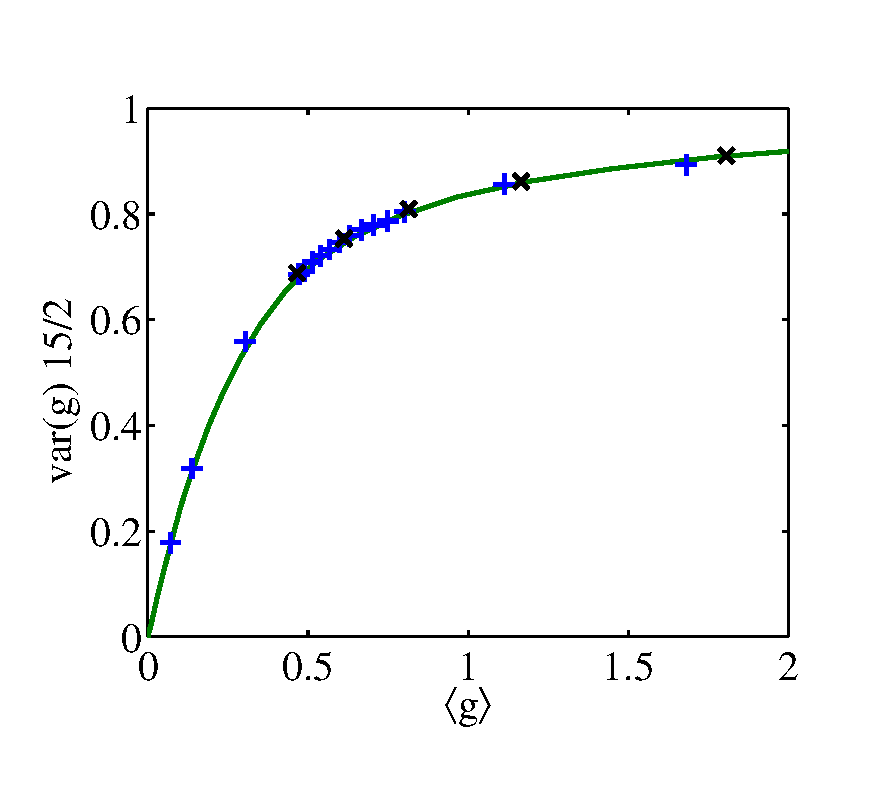
\includegraphics{chapters/Near-field_effects_in_wave_transport_through_in_disordered_waveguides/pictures/var_g_versus_g_no_closed_channels}}
}
\vskip -0.5cm
\caption[Variance of unitless conductance $g$ versus average $g$: comparison of quasi-1D numerical simulation results with non-linear sigma theory~\cite{2000_Mirlin} (solid green line) with no fitting parameters.]{Variance of unitless conductance $g$ versus average $g$: comparison of quasi-1D numerical simulation results with non-linear sigma theory~\cite{2000_Mirlin} (solid green line) with no fitting parameters. Waveguide results for with 10 (blue crosses) and 20 (black x) propagating channels and no evanescent channels when system length $L/\lambda$ is varied and $W/\lambda$ is constant. Very good agreement with the non-linear sigma model is found. Both numerical simulation and theory extend from diffusive ($g>1$) to localized ($g<1$) regime. The~$15/2$ coefficient for variance is due to waveguide geometry.}
% source of Mirlin's curve is Fig 6, page 349
% numerical data from 131.151.77.18/home/Q1D
\label{fig:vargversusg}
\end{figure}

When a finite number of evanescent channels are added, c.f.~Fig.~\ref{fig:vargversusgNCC}, the average conductance decreases. However, the ratio of average conductance to variance of conductance remains consistent with single parameter scaling %and with the theoretical prediction 
since variance also decreases. As more evanescent channels are included, the ratio monotonically decreases. %, while remaining on the curve which is based on no evanescent channels. 
Again, no fitting parameters are needed.
\begin{figure}
\vskip -0.5cm
\centerline{
\scalebox{.6}{\includegraphics{chapters/Near-field_effects_in_wave_transport_through_in_disordered_waveguides/pictures/var_g_versus_g}}}
\vskip -0.5cm
\caption[Same data as in Fig.~\ref{fig:vargversusg} ($N_p=10$ blue crosses and $N_p=20$ black x for varying system length $L$).]{Same data as in Fig.~\ref{fig:vargversusg} ($N_p=10$ blue crosses and $N_p=20$ black x for varying system length $L$). Added here is $L/\lambda=100$, $N_p=10$ with 0 to 10 evanescent channels (brown triangles) and $L/\lambda=200$, $N_p=10$ with 0 to 8 evanescent channels (red squares). No fitting parameters used. Here the primary conclusion, that evanescent channels renormalize $\ell_{\rm tmfp}$ while retaining the property of single parameter scaling, is apparent. }
% numerical data from 131.151.77.18/home/Q1D
\label{fig:vargversusgNCC}
\end{figure}
There are two important observations from Fig.~\ref{fig:vargversusgNCC}. First, the average conductance decreases when more evanescent channels are present because $\ell_{\rm tmfp}$ is renormalized. More channels are available at each scatterer for incident waves to scatter into, and there is increased propagation between adjacent scatterers. Analytically, renormalization of $\ell$ is accounted for by the folding procedure. Thus DMPK theory is valid even though no evanescent channels are included: when compared to other theories or experiment, $\ell_{\rm tmfp}$ is a fitting parameter. Therefore the effect of evanescent channels is undetectable. The second observation is that because $\ell_{\rm tmfp}$ is renormalized, single parameter scaling remains valid whether or not evanescent channels are included. Numerical models that do not include evanescent channels give valid transport descriptions for passive media. 

%When including a finite number of evanescent channels, it has been shown here no upper limit exists on the necessary number of evanescent channels that make a significant contribution to transport even with a minimum scatterer separation distance of $\sqrt{\frac{W \ L}{M}}$. 

In real experimental systems, scatterers are finite sized. This means there is a finite number of evanescent channels needed to describe the wave around a scatterer. The closer any two scatterers are, the more evanescent channels that are needed to accurately describe wave propagation. %This can be accounted computationally for by placing scatterers in the medium the maximum distance apart for a given density. This suggests that saturation (a finite number of evanescent channels needed to describe the transport) is attainable given that the parameters fit a constraint~\cite{1990_Bagwell}: \textbf{[What is $m$ here?]}
%\begin{equation}
%\frac{m}{ \hbar^2 \kappa_n}\frac{\gamma}{W} <<1.
%\end{equation}
% This is an incorrectly copied formula from Bagwell PRB 1990. page 358. We would need to translate from electronic to photonic
% \frac{m}{ \hbar^2} = (1/2) \frac{\omega^2}{c^2}
% to get the condition
% \frac{\frac{\omega^2}{2 c^2} \frac{1}{\kappa_{\parallel n}} \frac{\alpha}{W} << 1
% 20080616, book 3 of Ben's notes
Delta-function scatterers would be resolved by an infinite number of evanescent channels, but saturation would occur for finite-sized scatterers.

\begin{figure}
\vskip -0.5cm
\centerline{
\scalebox{.5}{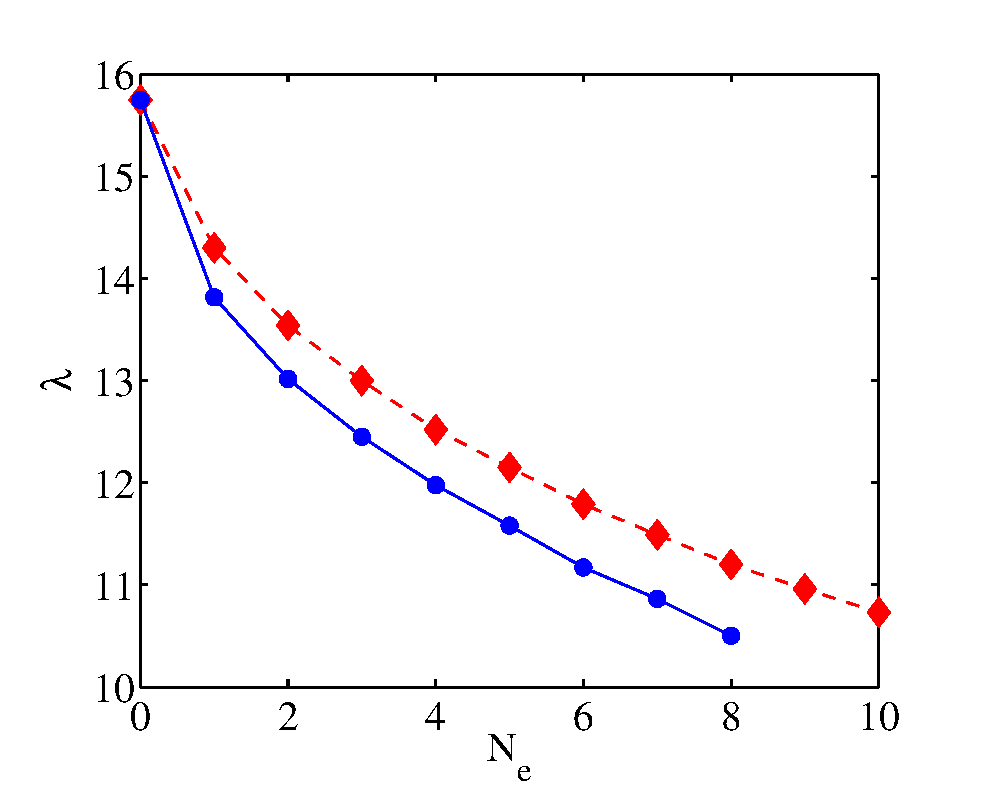
\includegraphics{chapters/Near-field_effects_in_wave_transport_through_in_disordered_waveguides/pictures/alpha1_W5_ltmfp_and_scat_versus_Nc_min_separation_05}}}
\vskip -0.2cm
\caption[Transport mean free path $\ell_{\rm tmfp}/\lambda$ (blue dots, solid line) renormalized as more evanescent channels ($N_e$) are included.]{Transport mean free path $\ell_{\rm tmfp}/\lambda$ (blue dots, solid line) renormalized as more evanescent channels ($N_e$) are included. % for $L/\lambda=200$, 10 propagating channels, $\alpha=1$ with minimum scatterer separation.
Red dashed line with diamonds is the scattering length defined by Eq.~\ref{eq:gb_lscat}. Both characteristic lengths are renormalized by inclusion of closed channels. No asymptotic value is apparent. 
}
\label{fig:lscat_ltmfp}
\end{figure}



Statements above concerning renormalization of $\ell_{\rm tmfp}$ above have only included the first two moments of conductance. To investigate whether all the moments are renormalized, we can find the entire distribution of conductance using the numerical model; c.f.~Fig.~\ref{fig:distgversusg}. When evanescent channels are included for a given waveguide geometry, the entire distribution changes (observed earlier as a change in both first and second moments). However, the system which includes evanescent channels has the same distribution as a longer waveguide with only propagating modes. Effectively, the presence of evanescent channels decreases $\ell_{\rm tmfp}$, which is equivalent to increasing system length $L$ since $g\propto~N_p\ell_{\rm tmfp}/L$. 
\begin{figure}
\vskip -0.5cm
\centerline{
\scalebox{.55}{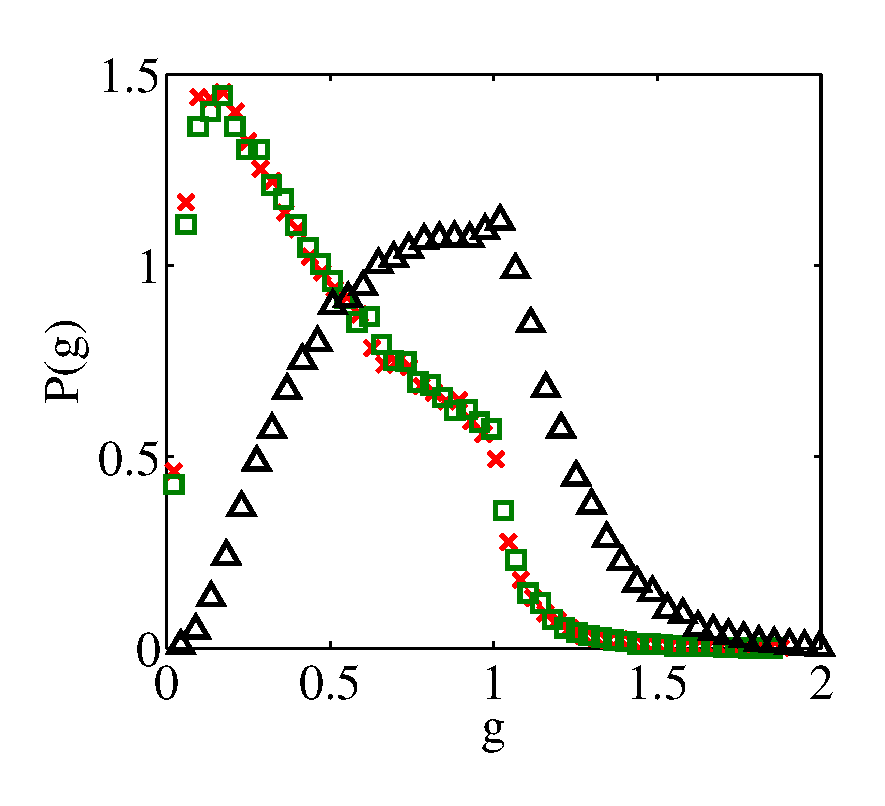
\includegraphics{chapters/Near-field_effects_in_wave_transport_through_in_disordered_waveguides/pictures/dist_g_vs_g_different_symbols_no_L600}}}
\vskip -0.5cm
\caption[Distribution of unitless conductance~$P(g)$ for three waveguides; each with 10 propagating channels.]{Distribution of unitless conductance~$P(g)$ for three waveguides; each with 10 propagating channels.  $P(g)$ from numerical simulation of waveguide system length $L/\lambda=200$ with no evanescent channels, black triangles is significantly distinct from $P(g)$ for same geometry and 8 evanescent channels (red x). However, the system with evanescent channels is equivalent to a longer system, $L/\lambda=300$, since $P(g)$ matches (green squares). The inclusion of evanescent channels renormalizes $\ell_{\rm tmfp}$ to be shorter, which is the equivalence of having a longer waveguide.}
% numerical data from 131.151.77.18/home/Q1D
\label{fig:distgversusg}
\end{figure}


%%%%%%%%%%%%%%%%%%%%%%%%%%%%%%%%%%%%%%%%%%%%%%%%%%%%%%%%%%%%%%%%%%%%%%%%%%%%%%
\section{CONCLUSION}
%%%%%%%%%%%%%%%%%%%%%%%%%%%%%%%%%%%%%%%%%%%%%%%%%%%%%%%%%%%%%%%%%%%%%%%%%%%%%%

The characteristic length for transport properties in random media with multiple scattering is $\ell_{\rm tmfp}$. Using analytical and computational analysis we have shown the renormalization of $\ell_{\rm tmfp}$ due to evanescent channels. For the analytical portion, the transfer matrix folding technique used by Bagwell and coworkers for single scatterers extends to multiple scatterers, which include density information. Thus $\ell_{\rm tmfp}$ is renormalized due to evanescent channels. 

Using a numerical transfer-matrix model of quasi-1D waveguides with densely packed, randomly-placed scatterers the effect of evanescent channels on conductivity was simulated. The number of matrices multiplied is limited by numerical accuracy, and has been extended using self-embedding technique~\cite{1999_yamilov_selfembed}. Transfer matrices can include a finite number propagating and evanescent channels. The number of evanescent channels was varied and single parameter scaling remained valid. Comparison with theoretical predictions agreed with no fitting parameters. However, the first and second moments of conductance decreased as more  evanescent channels were added. This can be attributed to the shorter $\ell_{\rm tmfp}$. 

The distribution of conductance changes when the number of evanescent channels is varied but is equivalent to a system with no evanescent channels and longer $L$ or a shorter $\ell_{\rm tmfp}$. The renormalization of $\ell_{\rm tmfp}$ due to evanescent channels explains how DMPK theory, in which $\ell_{\rm tmfp}$ is used as a fitting parameter, can agree with experimental measurements which necessarily include evanescent channels.

The results of our \textit{ab initio} numerical model are be explained by the folding procedure which analytically reduces the rank of transfer matrices to propagating channels only. We demonstrated renormalization applies to multiple scatterers, thus including interaction between scatterers, by finding $\ell_{\rm tmfp}$ as a function of the number of evanescent channels. Folding a single scatterer matrix renormalizes $\ell$, but inclusion of multiple scatterers is necessary to renormalize $\ell_{\rm tmfp}$. Since single parameter scaling is valid and average conductance is $g \propto N \ell_{\rm tmfp}/L$, then the entire distribution of conductance is reshaped. 

These effect of evanescent channels on transport properties is expected to be important in media with gain. We have shown using numerical simulations that evanescent channels renormalize $\ell_{\rm tmfp}$, which includes interaction between scatterers. 

% \newpage
%
% \begin{appendices}
% 
%   \renewcommand{\theequation}{A-\arabic{equation}}
%   % redefine the command that creates the equation no.
%   \setcounter{equation}{0}  % reset counter 
% 
% \include{appendix_derivation_single_scatterer_transfer_matrix}
% 
%   \renewcommand{\theequation}{B-\arabic{equation}}
%   % redefine the command that creates the equation no.
%   \setcounter{equation}{0}  % reset counter 
% 
% \include{appendix_derivation_folding_one_scattering_matrix}
% 
%   \renewcommand{\theequation}{C-\arabic{equation}}
%   % redefine the command that creates the equation no.
%   \setcounter{equation}{0}  % reset counter 
% 
% \include{appendix_derivation_folding_two_scatterers}
% 
%   \renewcommand{\theequation}{D-\arabic{equation}}
%   % redefine the command that creates the equation no.
%   \setcounter{equation}{0}  % reset counter 
% 
% \include{appendix_derivation_folding_two_scatterers_matrices}
% \newpage
% \end{appendices}
% 
% \bibliographystyle{apsrevM}
% %\bibliographystyle{unsrt} % order the citations according to when they show up in the paper
% \bibliography{../../Bibliography/latex_bibliography}

% also need to cite 1991_Mello_Tomsovic

%useful sites for latex formatting
%  http://en.wikibooks.org/wiki/LaTeX/Mathematics
%  http://www.tex.ac.uk/cgi-bin/texfaq2html?label=appendix
%conventions:
%  Fig.~\ref{fig:
%  Eq.~\ref{
%  Ref.~\cite{
%\end{document}
%eof
